
A comparison of force response in the form of normalized lift and drag forces is shown in Figures \ref{fig:lift_zonal_adapt} and \ref{fig:drag_zonal_adapt}, respectively. Normalized lift compares well for all the meshes considered. Normalized drag is similar for the Mza2 and Mza3 series meshes, but shows differences as compared to the M0 and Mza1 series meshes. Maximum drag in the advancing phase is observed around $\psi=72^\circ$, with Mza3 series meshes predicting slightly higher drag than the Mza2 series meshes, followed by the Mza1 series and M0 meshes. Major differences in drag between different meshes are observed specifically between phases $\psi=160^\circ$ and $\psi=240^\circ$. Between these phases, the Mza2 and Mza3 series meshes compare well with each other, whereas the M0 and Mza1 series meshes predict lower drag than the Mza2 and Mza3 series meshes. Note that normalized lift and drag response remains unaffected with changes in the spanwise mesh resolution for the same in-plane mesh.

\begin{figure}[H]
\centering

\begin{subfigure}[b]{0.7\textwidth}
\centering
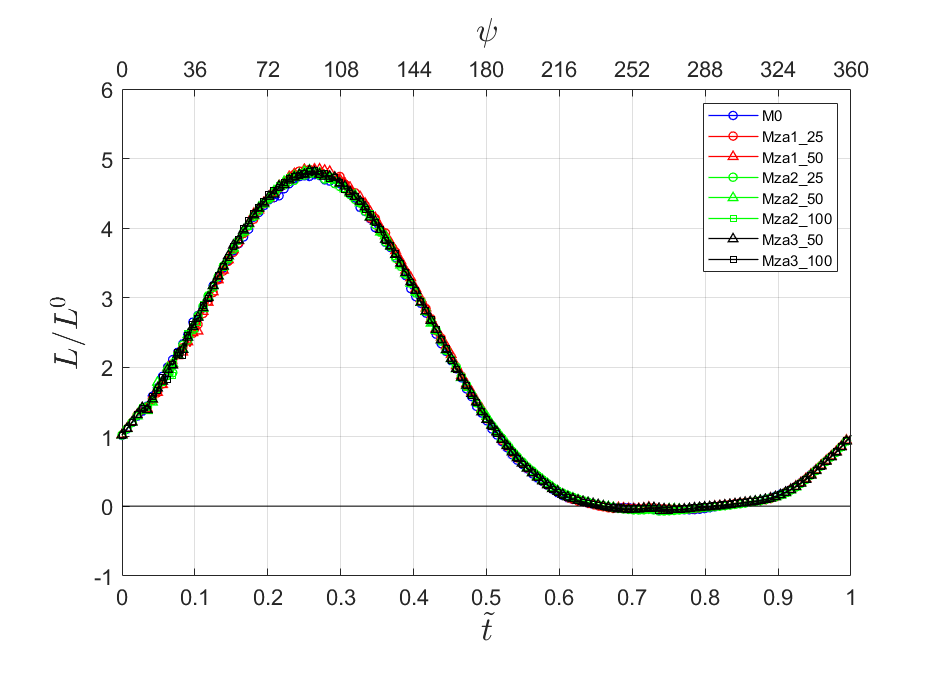
\includegraphics[width=1\textwidth]{figures/zonal_adapt_results/force_response/Lift.png}
\caption{Normalized lift}
\label{fig:lift_zonal_adapt}
\end{subfigure}
\begin{subfigure}[b]{0.7\textwidth}
\centering
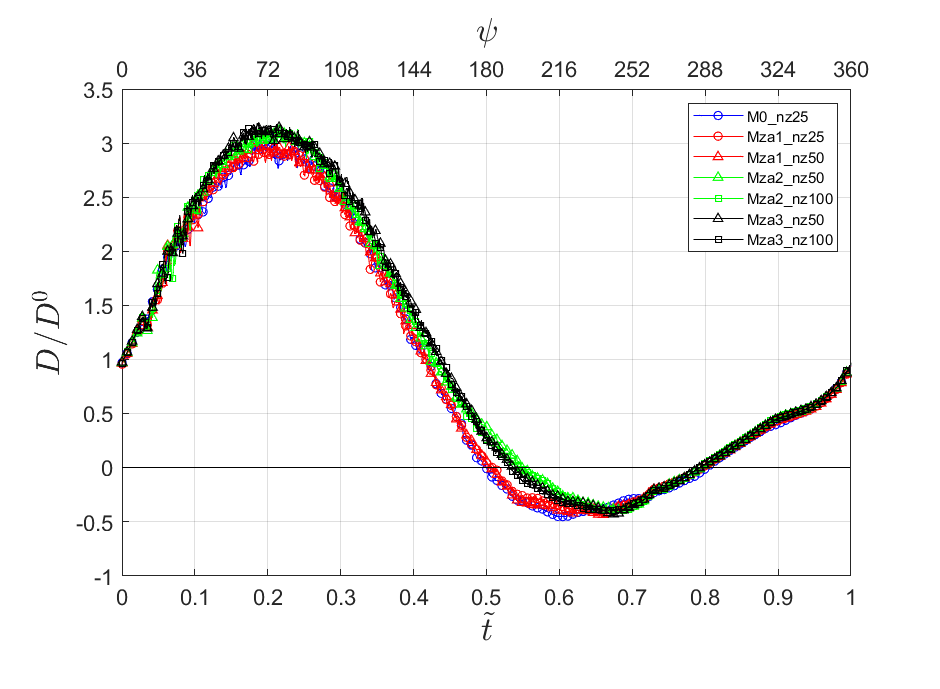
\includegraphics[width=1\textwidth]{figures/zonal_adapt_results/force_response/Drag.png}
\caption{Normalized drag}
\label{fig:drag_zonal_adapt}
\end{subfigure}

\label{fig:force_response_zonal_adapt}
\caption{Adaptive LES at $Re=40,000$: normalized forces}
\end{figure}